\chapter{Système RAG et assistance intelligente}

\section*{Introduction}
\addcontentsline{toc}{section}{Introduction}

Le classifieur du chapitre précédent affecte une catégorie à chaque ticket. Savoir qu'une demande
relève de la catégorie \emph{Microsoft} oriente son affectation sans dire comment la traiter. Ce
chapitre construit le second volet de la solution : un moteur qui retrouve dans l'historique les
tickets comparables et présente leur résolution à l'administrateur. La redondance du corpus, qui a
bridé le classifieur, devient ici un atout, puisque cinquante-huit scénarios réinstanciés rendent
probable qu'un nouveau ticket ressemble à un ticket déjà résolu.

Trois moteurs ont été construits et comparés sous un protocole unique, recherche lexicale,
recherche sémantique et leur combinaison, complétés par un modèle de langage exécuté sur
l'infrastructure du service. Deux résultats et deux limites sont annoncés d'emblée.

\begin{puces}
  \item Le moteur hybride, celui qui est servi, obtient la meilleure précision à trois passages,
        0,3542 contre 0,2917 pour le sémantique seul.
  \item Sa similarité moyenne, 0,3551, n'atteint jamais le seuil de pertinence de 0,50 : aucune des
        quatre-vingts requêtes d'évaluation n'a été servie autrement que par le mécanisme de repli
        (section~\ref{sec:seuil5}).
  \item Aucun jeu d'évaluation annoté n'existe pour la recherche, si bien que les mesures reposent
        sur un protocole indicatif (section~\ref{sec:eval5}).
  \item Le découpage anti-fuite place les scénarios du jeu de test hors de la base : aucune requête
        d'évaluation n'admet de bonne réponse, et les valeurs constituent un plancher
        (section~\ref{sec:antifuite5}).
\end{puces}

\section{Présentation du système RAG}

Le principe de la génération augmentée par récupération, introduit par Lewis et
ses coauteurs~\cite{lewis2020} et depuis largement décliné~\cite{gao2023}, a été exposé au
chapitre~2. Sa déclinaison ici tient en peu de mots : une demande entrante est comparée aux résolutions déjà consignées, les
plus proches sont retenues, un modèle de langage les reformule avant affichage. Le système ne
produit aucune connaissance nouvelle, il retrouve et met en forme ce que le service sait déjà.

La figure~\ref{fig:chaine5} donne la chaîne servie sur deux niveaux. En haut le parcours de
recommandation, du ticket entrant à la réponse reformulée ; en bas le parcours d'alimentation, par
lequel une solution validée par un administrateur revient enrichir la base.

\begin{figure}[!htbp]
\centering
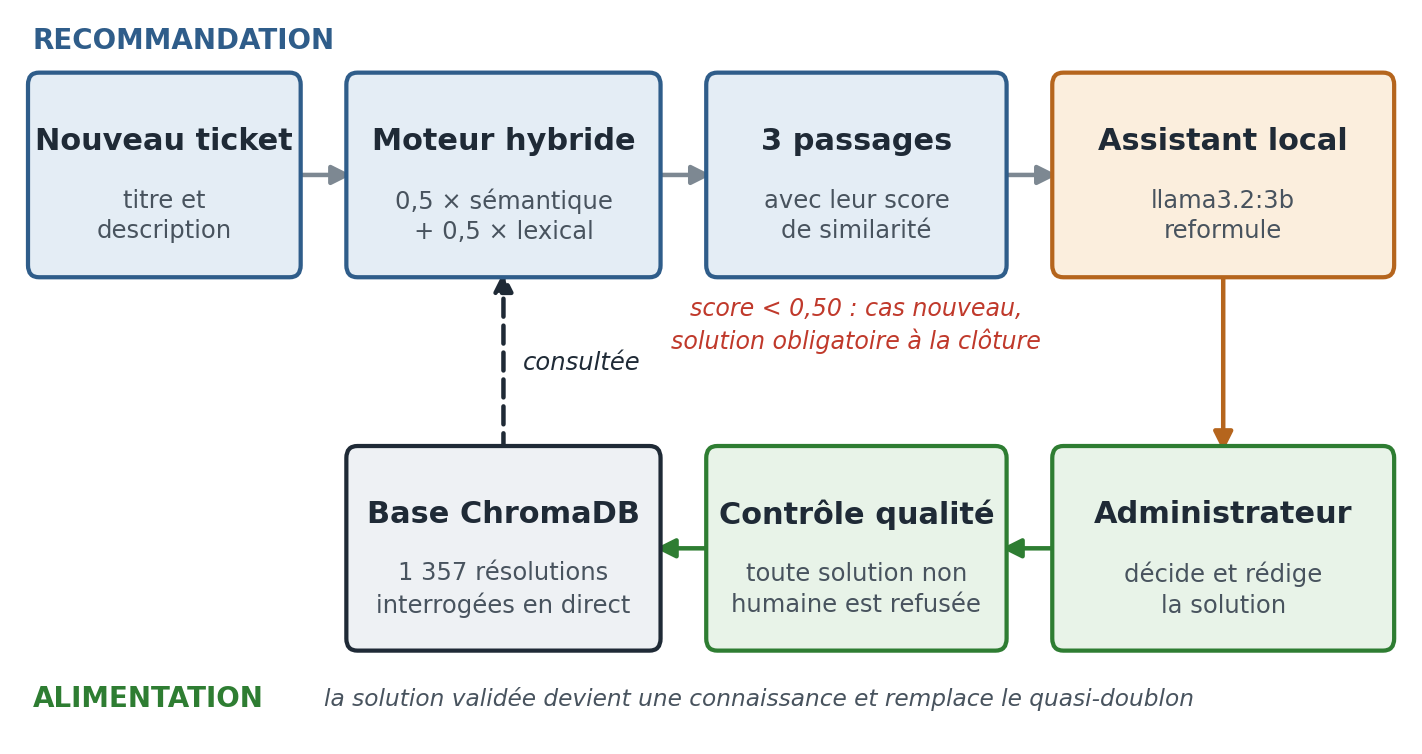
\includegraphics[width=\textwidth]{ch05_chaine_rag.png}
\caption{Chaîne servie du système RAG}
\label{fig:chaine5}
\end{figure}

\FloatBarrier

\section{Construction de la base de connaissances}

\subsection{Composition de la base}

La base est produite par le module de découpage du corpus, au même moment que les jeux
d'entraînement et de test. Elle retient tout ticket du jeu d'entraînement dont le champ
\emph{Résolution\,/\,Motif} est renseigné, soit \textbf{1\,357 tickets} sur les huit catégories du
référentiel, sans restriction au statut \emph{Résolu}.

\begin{table}[!htbp]
\centering
\styletableau
\caption{Composition de la base de connaissances par statut de ticket}
\label{tab:kb5}
\begin{tabular}{|Lp{4.6cm}|Cp{2.4cm}|Lp{6.4cm}|}
\hline
\rowcolor{enteteTab}
\textbf{Statut du ticket} & \textbf{Effectif} & \textbf{Ce que le champ contient} \\
\hline
Rejeté & 363 & Le motif du refus, qui vaut réponse pour une demande semblable \\
\hline
Résolu & 358 & La procédure appliquée \\
\hline
Problème & 237 & Le diagnostic posé, la cause identifiée \\
\hline
Prise en charge & 236 & L'action engagée et son état d'avancement \\
\hline
En attente & 163 & L'élément manquant qui bloque le traitement \\
\hline
\rowcolor{enteteTab}
\textbf{Total} & \textbf{1\,357} & \\
\hline
\end{tabular}
\end{table}

Un rejet documenté répond à une question réelle du demandeur, et l'écarter priverait la base d'un
quart de sa matière. La contrepartie est admise : un ticket \emph{En attente} décrit un blocage
plutôt qu'une solution. Nous avons retenu la couverture large parce que l'administrateur reste seul
décideur.

Ces documents sont conservés dans ChromaDB, que le service applicatif interroge directement, et
indexés selon les deux représentations de la section suivante. La base n'est pas figée : la
section~\ref{sec:boucle5} montre comment une solution validée en exploitation vient s'y ajouter.

\subsection{Format des résolutions}

Les textes retenus sont courts, de longueur médiane \textbf{12 mots} et d'étendue 7 à 16 mots.

\begin{quote}
\og Vérifier les entrées DNS, vider le cache DNS client, forcer l'enregistrement du serveur. \fg{}
\end{quote}

Une résolution de douze mots énumère des gestes sans les expliquer. Elle vaut comme repère pour un
technicien du domaine, non comme procédure autonome. Cette brièveté limite ce qu'un modèle de
langage peut en tirer, puisqu'il n'a rien à résumer, et explique que l'assistant de la
section~\ref{sec:llm5} soit conçu pour reformuler. Le moteur épargne une recherche manuelle dans
plusieurs milliers de lignes, il ne remplace pas l'expertise de l'administrateur.

\subsection{Volume indexé et diversité réelle des réponses}
\label{sec:diversite5}

Le décompte de 1\,357 tickets décrit un volume, non une richesse. Les tickets indexés portent
\textbf{46 résolutions distinctes} pour 46 titres distincts, dans une correspondance exacte : à
chaque scénario du corpus d'entraînement répond une résolution et une seule, réinstanciée en
médiane 31 fois, de 4 à 49 fois selon les cas.

\begin{table}[!htbp]
\centering
\styletableau
\caption{Nombre de résolutions distinctes par catégorie dans la base de connaissances}
\label{tab:diversite5}
\begin{tabular}{|Bp{3.4cm}|Cp{3.0cm}|Bp{3.4cm}|Cp{3.0cm}|}
\hline
\rowcolor{enteteTab}
\textbf{Catégorie} & \textbf{Réponses} & \textbf{Catégorie} & \textbf{Réponses} \\
\hline
Applicatifs & 8 & Microsoft & 6 \\
\hline
Réseau & 8 & Communication & 5 \\
\hline
Backup & 6 & Système & 5 \\
\hline
Infrastructure & 4 & Sécurité & 4 \\
\hline
\end{tabular}
\end{table}

La conséquence est double. Un incident récurrent trouve la réponse exacte que le service a déjà
appliquée, usage précisément visé ; un incident inédit ne trouve rien, la base ne couvrant que
quarante-six situations. Quatre réponses pour toute la catégorie \emph{Sécurité} laissent peu de
marge à la variété des incidents que ce mot recouvre.

\subsection{Le coût de la contrainte anti-fuite}
\label{sec:antifuite5}

Aucun ticket du jeu de test ne figure dans la base. Sans cette restriction, une requête
d'évaluation s'y retrouverait elle-même avec une similarité proche de~1, et toute mesure de qualité
deviendrait sans objet.

Son coût est plus lourd qu'il n'y paraît. Le découpage étant groupé par titre, les 58 scénarios du
corpus se répartissent en deux ensembles \textbf{disjoints}, 46 pour la base et 12 pour le jeu de
test. Les 356 tickets de ce jeu appartiennent donc tous à des scénarios dont \textbf{aucune
résolution ne figure dans la base} : aucune requête d'évaluation n'admet de bonne réponse, et le
moteur ne peut au mieux que proposer le voisin le plus plausible venu d'un autre scénario. Deux
règles de lecture en découlent.

\begin{puces}
  \item Les valeurs de la section~\ref{sec:resultats5} constituent un \textbf{plancher}, non une
        estimation du service rendu en exploitation, où un incident récurrent retrouve les
        instances antérieures de son propre scénario.
  \item Les scores de similarité mesurés sont bas par construction, ce dont la
        section~\ref{sec:seuil5} tire les conséquences.
\end{puces}

\FloatBarrier

\section{Mise en œuvre de la recherche}

\subsection{Recherche lexicale}

Le premier moteur applique la représentation vectorielle du chapitre~4, pondération TF-IDF sur cinq
mille descripteurs en unigrammes et bigrammes, avec classement par similarité cosinus dans l'espace
des documents indexés.

Ce moteur trouve un ticket lorsque la demande et la résolution partagent des mots, ce qui le rend
précis sur les formulations exactes et aveugle au reste. La limite n'est pas théorique dans un
corpus rédigé par des utilisateurs : une même panne de messagerie se dit \og je ne reçois plus mes
mails \fg{}, \og la synchronisation échoue \fg{} ou \og Outlook ne se connecte plus \fg{}, sans
qu'aucun mot commun ne subsiste.

\subsection{Recherche sémantique}

Le second moteur encode chaque ticket par un modèle de plongements de phrases,
\texttt{paraphrase-multilingual-mpnet-base-v2}, qui produit un vecteur de 768 dimensions. Ce modèle
traite le français sans traduction intermédiaire, a été entraîné à rapprocher des paraphrases et
s'exécute sans accélération graphique.

L'index est construit avec FAISS, en produit scalaire sur vecteurs normalisés. Cette normalisation
rend le produit scalaire égal au cosinus, donc la similarité bornée entre $-1$ et~$1$ et comparable
d'une requête à l'autre. Un index global est complété par un index par catégorie, ce qui permet de
restreindre la recherche lorsque la catégorie prédite est jugée fiable.

\subsection{Recherche hybride}

Le troisième moteur interroge les deux précédents et fusionne leurs scores. Nous retenons une
combinaison linéaire des scores plutôt qu'une fusion par les rangs~\cite{cormack2009}, afin de
conserver une échelle de similarité comparable à celle du seuil de pertinence :

\[
\text{score}_{\text{hybride}} = \alpha \cdot \text{score}_{\text{sémantique}}
+ (1 - \alpha) \cdot \text{score}_{\text{lexical}}
\]

Le paramètre $\alpha$ vaut 0,5 dans la configuration servie. Chaque sous-moteur remonte quinze
candidats sans filtrage, la fusion s'applique ensuite, le filtrage par seuil intervient en dernier,
ordre qui évite qu'un ticket écarté trop tôt soit perdu pour la fusion. L'intention est de réunir
la tolérance à la reformulation du sémantique et la précision du lexical sur les tickets répétés à
l'identique ; la section~\ref{sec:seuil5} montre l'effet secondaire que cette fusion produit.

\subsection{Comparaison des approches}

Ce qui sépare les trois moteurs tient moins à leur qualité qu'à ce que chacun sait voir.

\begin{table}[!htbp]
\centering
\styletableau
\caption{Ce que chaque moteur retrouve, et ce qui lui échappe}
\label{tab:comparaison5}
\begin{tabular}{|Bp{2.4cm}|Lp{5.6cm}|Lp{5.4cm}|}
\hline
\rowcolor{enteteTab}
\textbf{Moteur} & \textbf{Ce qu'il retrouve} & \textbf{Ce qui lui échappe} \\
\hline
Lexical & Les tickets qui emploient les mêmes mots que la demande & Un incident décrit avec un
autre vocabulaire \\
\hline
Sémantique & Les tickets qui décrivent le même incident, quels que soient les mots & Les
formulations exactes que le lexical classe en tête \\
\hline
Hybride & Les deux, par fusion à poids égal & Rien de plus, mais son échelle de score n'est plus
celle sur laquelle le seuil a été calibré \\
\hline
\end{tabular}
\end{table}

\FloatBarrier

\section{Évaluation du RAG}
\label{sec:eval5}

\subsection{Protocole et approximation de la pertinence}

La campagne interroge les trois moteurs avec quatre-vingts requêtes du jeu de test, en demandant
trois passages, et les sollicite exactement comme le fait l'application, mécanisme de repli
compris. Quatre indicateurs sont calculés.

\begin{puces}
  \item \textbf{Précision à trois passages} : proportion de passages pertinents parmi les trois
        retournés.
  \item \textbf{Rang réciproque moyen} : récompense un premier passage pertinent placé tôt.
  \item \textbf{Gain cumulé actualisé normalisé} : pondère chaque passage pertinent par sa position
        et rapporte le résultat au classement idéal.
  \item \textbf{Similarité moyenne} : valeur brute rendue par le moteur, comparée au seuil de
        pertinence.
\end{puces}

Décider si un passage est pertinent suppose de savoir ce qui l'est, information qui n'existe pas :
aucun jeu de référence annoté n'a été constitué. Le protocole considère comme pertinent tout
passage de la même catégorie que la requête. La règle est grossière, deux tickets \emph{Réseau}
pouvant décrire des incidents sans rapport.

Une raison plus contraignante que l'absence d'annotation impose cette approximation. Les scénarios
du jeu de test et ceux de la base sont disjoints (section~\ref{sec:antifuite5}), si bien qu'une
définition stricte donnerait \textbf{zéro} pour les trois moteurs, la bonne réponse étant absente
de l'index par construction. Le fichier de résultats porte cet avertissement : les valeurs servent
à \textbf{comparer les trois moteurs entre eux}, elles ne mesurent pas la pertinence perçue par un
administrateur. Le rappel à trois passages n'est pas publié pour la même raison, l'ensemble des
passages pertinents étant la catégorie entière, soit plusieurs centaines de tickets.

\subsection{Dimensions non couvertes par la campagne}

Deux dimensions échappent entièrement à la campagne, et le fichier de résultats les énumère.

\begin{puces}
  \item La \textbf{fidélité de la génération}. Le chemin de classification n'appelle aucun modèle
        de langage, et la reformulation destinée à l'administrateur constitue un appel séparé et
        facultatif, qui supposerait un protocole distinct.
  \item L'\textbf{utilité perçue}. Elle demanderait un retour explicite de l'administrateur sur
        chaque recommandation, que l'interface ne collecte pas.
\end{puces}

La commande d'évaluation produit sur option le gabarit d'annotation, soit quatre-vingts requêtes et
leurs dix meilleurs candidats. Le travail restant se compte en une demi-journée d'annotation par un
administrateur du service, et la conclusion générale porte cette lacune aux perspectives.

\FloatBarrier

\subsection{Résultats mesurés}
\label{sec:resultats5}

\begin{figure}[!htbp]
\centering
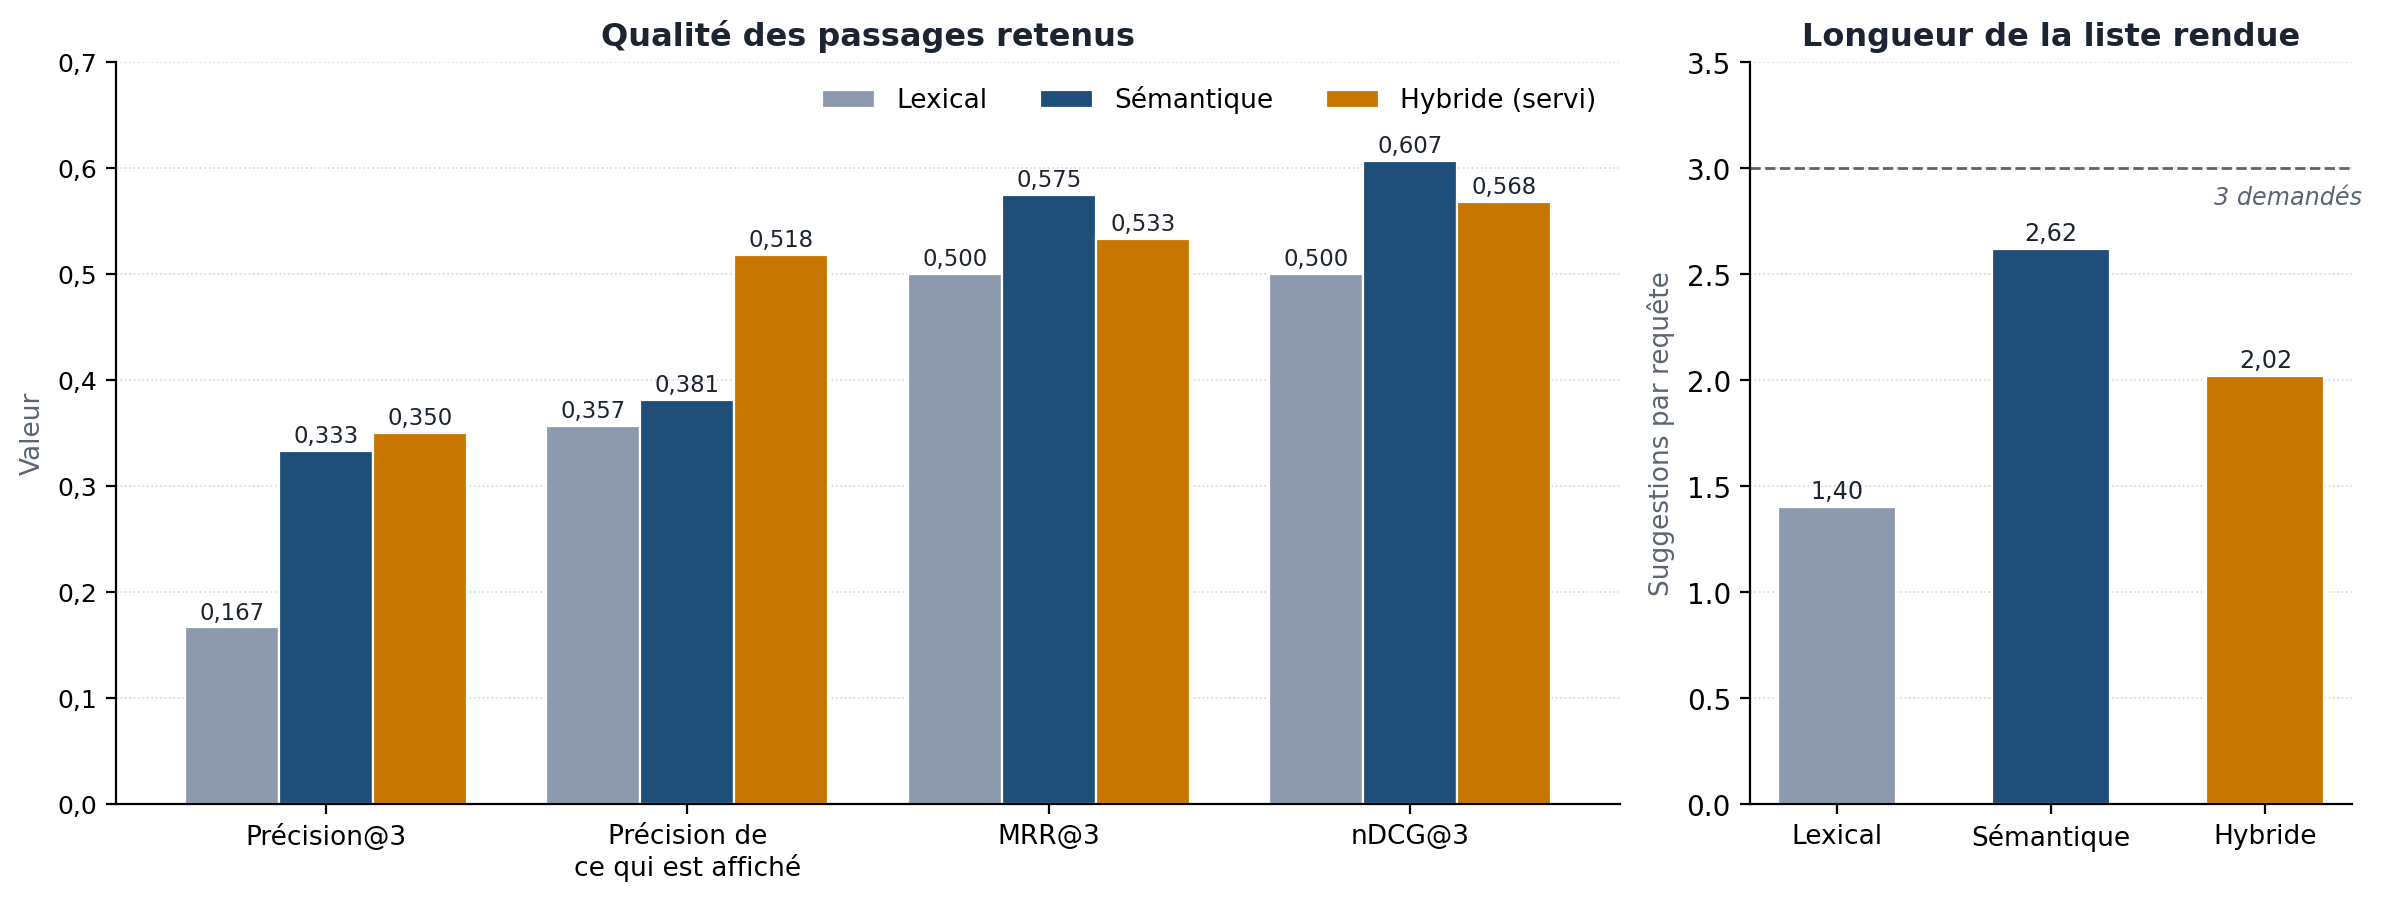
\includegraphics[width=\textwidth]{ch05_moteurs.png}
\caption{Comparaison des trois moteurs de recherche, 80 requêtes du jeu de test, trois passages
demandés}
\label{fig:moteurs5}
\end{figure}

\begin{table}[!htbp]
\centering
\styletableau
\caption{Comparaison des trois moteurs de recherche sous le protocole d'approximation}
\label{tab:moteurs5}
\begin{tabular}{|Bp{3.0cm}|Cp{2.0cm}|Cp{1.8cm}|Cp{1.8cm}|Cp{2.2cm}|Cp{1.8cm}|}
\hline
\rowcolor{enteteTab}
\textbf{Moteur} & \textbf{Précision @3} & \textbf{MRR @3} & \textbf{nDCG @3} &
\textbf{Similarité moyenne} & \textbf{Taux de repli} \\
\hline
Lexical & 0,1542 & 0,4354 & 0,4391 & 0,2117 & 1,000 \\
\hline
Sémantique & 0,2917 & \textbf{0,5813} & \textbf{0,5960} & \textbf{0,6099} & 0,0125 \\
\hline
Hybride (servi) & \textbf{0,3542} & 0,5375 & 0,5754 & 0,3551 & 1,000 \\
\hline
\end{tabular}
\end{table}

Le moteur sémantique domine le lexical sur les quatre indicateurs, l'écart le plus net portant sur
la précision, de 0,1542 à 0,2917, et sur la similarité moyenne, de 0,2117 à 0,6099. Dans un corpus
rédigé en langage libre, la proximité de sens retrouve des cas que le partage de vocabulaire
manque.

Le moteur hybride obtient la meilleure précision mesurée, 0,3542, quand ses indicateurs de
classement restent derrière le sémantique, 0,5375 contre 0,5813 pour le rang réciproque et 0,5754
contre 0,5960 pour le gain cumulé. La précision compte les passages pertinents sans considérer leur
ordre, tandis que les deux autres récompensent le fait de placer le bon passage en tête : la fusion
fait entrer dans le trio de tête des passages que le sémantique écartait, en ordonnant l'ensemble
un peu moins bien. Pour un usage où l'administrateur lit les trois propositions, la précision est
l'indicateur qui compte, ce qui justifie le choix du moteur hybride.

\subsection{Le seuil que le moteur servi n'atteint jamais}
\label{sec:seuil5}

Le paramétrage fixe un seuil de pertinence à 0,50 et un seuil de repli à 0,20. Une requête dont
aucun passage n'atteint 0,50 n'est servie que par le repli, et la dernière colonne du
tableau~\ref{tab:moteurs5} compte ces requêtes : 0,0125 pour le sémantique, soit une requête sur
quatre-vingts, et \textbf{1,000} pour l'hybride.

Le mécanisme est arithmétique. Le score hybride est la moyenne du score sémantique, 0,6099, et du
score lexical, 0,2117, soit 0,3551, très en dessous de 0,50. Atteindre le seuil avec un score
lexical de l'ordre de 0,21 exigerait un score sémantique d'environ 0,79, valeur que le moteur
sémantique lui-même n'atteint pas en moyenne. Le seuil a donc été calibré sur l'échelle du moteur
sémantique puis conservé tel quel, alors que la fusion change l'échelle des scores en même temps
que le classement.

Un second facteur pèse sur ces valeurs sans se confondre avec le premier : les scores sont bas en
partie parce qu'aucune requête d'évaluation n'a sa réponse dans la base
(section~\ref{sec:antifuite5}). Le diagnostic d'échelle reste valable indépendamment, la moyenne
avec un score lexical borné vers 0,21 divisant par deux l'écart au seuil.

La conséquence sur l'application est directe. Le module de traitement des tickets utilise le même
seuil de 0,50 pour décider qu'un ticket constitue un \emph{cas nouveau}, pour lequel
l'administrateur doit rédiger la solution appliquée avant de clore : un score systématiquement
inférieur revient à traiter tout ticket comme un cas nouveau. L'effet garantit que la base est
alimentée à chaque clôture, ce qui est l'intention de la boucle décrite à la
section~\ref{sec:boucle5}, mais il l'obtient par accident de calibrage et prive le seuil de sa
fonction de discrimination. Deux corrections sont envisageables, que nous énonçons sans trancher
faute de trafic réel : relever $\alpha$ pour rapprocher l'échelle hybride de l'échelle sémantique,
ou fixer un seuil propre au moteur hybride.

\subsection{Une mesure ancienne à ne pas citer}

Les métadonnées du moteur sémantique rapportent une similarité moyenne de 0,9321 contre 0,7646 pour
la recherche lexicale. Un lecteur qui ouvre ces fichiers rencontrera ces nombres, que deux
précisions écartent de toute citation.

La quantité mesurée n'est pas celle du tableau~\ref{tab:moteurs5} : il s'agit de la similarité du
\emph{meilleur} passage, quand la campagne rapporte la similarité moyenne des \emph{trois} passages
retenus. Et cette mesure a été conduite sur un index de \textbf{476 documents}, à un stade
antérieur du projet, alors que l'index servi en contient 1\,357. La campagne rapportée au
tableau~\ref{tab:moteurs5} reste la référence unique de ce chapitre, parce qu'elle mesure les trois
moteurs sous un protocole identique et sur l'index réellement servi.

\FloatBarrier

\section{Intégration du LLM}
\label{sec:llm5}

\subsection{Un modèle exécuté sur site}

Les quarante-six résolutions du corpus initial sont propres et uniformes
(section~\ref{sec:diversite5}). Il n'en va pas de même des solutions saisies en exploitation :
rédigées dans un champ libre au fil du traitement, elles portent les fautes et les abréviations
d'une saisie rapide, et ce sont pourtant elles qui alimentent la base. Un modèle de langage qui les
reformule en français professionnel homogénéise la présentation quelle que soit la qualité de la
saisie.

Le choix d'exécuter ce modèle sur l'infrastructure du service découle d'une contrainte du client.
Un ticket contient le nom du demandeur, sa filiale, parfois des éléments d'architecture du système
d'information. Les règles internes de confidentialité d'\otbs~\cite{otbs-integration} encadrent la
circulation de ces contenus, et les transmettre à un service tiers aurait supposé une démarche
contractuelle et un accord de traitement qui dépassent le cadre d'un projet de fin d'études.

Aucune donnée de ticket ne quitte donc l'infrastructure, contrainte qui exclut les modèles
accessibles uniquement par interface distante. Le modèle retenu est \texttt{llama3.2:3b}, servi par
Ollama : trois milliards de paramètres tiennent en mémoire sur une machine de bureau tout en
produisant un français correct. La carte graphique disponible, une NVIDIA GeForce MX130 de 2~Go, ne
suffit pas à le charger entièrement en mémoire vidéo ; l'exécution se fait par défaut sur le
processeur, un fichier de composition optionnel activant l'accélération.

Sur processeur, le premier appel demande environ quatre-vingt-quinze secondes et les suivants de
dix-huit à vingt. L'accélération graphique ramène ces durées à quarante-sept et treize secondes, en
occupant 770~Mo des 2\,048~Mo disponibles. Le gain apporté par la carte reste de l'ordre de trente
pour cent, précisément parce que le modèle n'y tient pas entièrement. L'accélération n'est pas
activée par défaut, afin qu'un poste dépourvu de carte compatible démarre sans échec.

\subsection{Conception du prompt}

Un modèle de trois milliards de paramètres suit mal des consignes abstraites. L'instruction système
impose un format en trois parties :

\begin{puces}
  \item une phrase d'introduction annonçant le nombre de tickets trouvés ;
  \item une ligne par ticket au format exact \og \textbf{Ticket \#identifiant (Score : x\%
        - catégorie) :} \fg{} suivie d'une phrase de reformulation ;
  \item une question finale invitant l'administrateur à désigner le cas retenu.
\end{puces}

Elle interdit explicitement de recopier le texte brut et de produire autre chose. Un exemple
complet, injecté dans l'historique de conversation avec une requête fictive et la réponse attendue,
complète ces consignes ; cet amorçage par l'exemple améliore sensiblement le respect du format et a
introduit le défaut que la sous-section suivante expose. Un second prompt gouverne le mode
conversationnel, où l'administrateur pose des questions de suivi sur le ticket courant, sous les
mêmes règles de non-invention.

\subsection{Garde-fous et repli}

Un ticket avait été clos avec, dans le champ \emph{solution appliquée}, le texte de la synthèse
générée par l'assistant lui-même, collé par erreur depuis le panneau d'affichage. Redevenu candidat
pour un ticket suivant, ce contenu qui ressemblait déjà à une synthèse a conduit le modèle à
continuer le motif et à produire deux tickets inexistants, reprenant les identifiants \#1042 et
\#985 de l'exemple d'amorçage.

\begin{table}[!htbp]
\centering
\styletableau
\caption{Garde-fous appliqués à la reformulation}
\label{tab:garde5}
\begin{tabular}{|Bp{3.2cm}|Lp{5.2cm}|Lp{5.0cm}|}
\hline
\rowcolor{enteteTab}
\textbf{Garde-fou} & \textbf{Mécanisme} & \textbf{Effet} \\
\hline
Assainissement en entrée & Une résolution qui présente la signature d'une synthèse déjà générée
est remplacée avant d'entrer dans le prompt & Le modèle ne reçoit plus de texte qui l'invite à
poursuivre un motif \\
\hline
Validation en sortie & Tout identifiant de ticket cité par le modèle est confronté à la liste des
candidats réellement fournis & Un identifiant inventé fait basculer l'affichage sur le
récapitulatif brut \\
\hline
Température basse & Le paramètre d'échantillonnage est fixé à 0,2 & La réponse suit de plus près
les données fournies \\
\hline
Plafond de production & La longueur de sortie est bornée à 400 unités lexicales & Le pire cas de
latence est borné \\
\hline
\end{tabular}
\end{table}

Le tableau~\ref{tab:garde5} rassemble les quatre garde-fous du module, dont les deux premiers ont
été ajoutés après cet incident et éprouvés en rejouant le scénario dans les deux sens, avec le
ticket contaminé comme cible puis comme candidat. Aucune invention n'a été observée depuis.

La limite doit être énoncée : la validation en sortie porte sur les identifiants, qui suivent un
format reconnaissable, et ne vérifie pas que le contenu reformulé reste fidèle à la résolution
d'origine. La conclusion générale reprend cet écart. La cause structurelle, une synthèse jamais
relue par un humain pouvant entrer dans la base, est fermée en amont par le contrôle qualité de la
section~\ref{sec:boucle5}.

L'appel au modèle reste facultatif par construction, puisqu'il intervient après le calcul et
l'affichage de la recommandation. Si le service est indisponible ou si l'appel dépasse le délai de
quatre-vingt-dix secondes, l'application retombe sur un récapitulatif brut des cas trouvés. Le
maintien du modèle en mémoire pendant trente minutes évite le rechargement entre deux appels
rapprochés, ce qui explique l'écart mesuré plus haut entre le premier appel et les suivants.

\FloatBarrier

\section{Apprentissage continu}
\label{sec:boucle5}

Le niveau inférieur de la figure~\ref{fig:chaine5} porte le parcours dont il est question ici.

\subsection{D'un journal à une base interrogée}

La première version archivait les tickets résolus dans une base documentaire légère que rien ne
relisait jamais : elle fonctionnait comme un journal, alimenté et jamais consulté, tandis que le
moteur continuait de travailler sur le corpus figé issu du découpage.

La migration vers ChromaDB a changé cette situation. La collection est désormais interrogée à
chaque recommandation, et une solution rédigée par un administrateur devient candidate dès le
ticket similaire suivant, ce qui a été vérifié en exploitation. Cette vérification a mis au jour un
défaut propre à l'exécution multi-processus, la collection étant mise en cache par processus : un
serveur ne voyait pas les écritures faites par l'autre. La correction porte sur la fraîcheur de la
collection entre processus, et l'incident est clos.

\subsection{Le contrôle qualité}

Un module de contrôle applique quatre règles avant indexation.

\begin{table}[!htbp]
\centering
\styletableau
\caption{Règles du contrôle qualité appliquées avant indexation}
\label{tab:qualite5}
\begin{tabular}{|Bp{3.6cm}|Cp{2.0cm}|Lp{7.6cm}|}
\hline
\rowcolor{enteteTab}
\textbf{Règle} & \textbf{Seuil} & \textbf{Ce qu'elle écarte} \\
\hline
Origine humaine & exigée & Une suggestion produite par l'assistant et jamais relue \\
\hline
Longueur minimale & 4 mots & Une mention de clôture sans contenu, du type \og ok \fg{} \\
\hline
Recouvrement avec la description & 0,90 & Une solution qui recopie l'énoncé du problème \\
\hline
Quasi-doublon & 0,95 & Une redite d'une connaissance déjà indexée, qui est alors remplacée \\
\hline
\end{tabular}
\end{table}

La règle d'origine humaine est la plus importante. Une suggestion produite par le système, quelle
que soit sa qualité apparente, ne peut devenir une connaissance de référence tant qu'un
administrateur ne l'a pas reprise à son compte. Elle ferme la voie d'auto-contamination : sans
elle, le système apprendrait de ses propres sorties et un écart introduit une fois se propagerait
de recommandation en recommandation.

\subsection{Le cycle de vie des connaissances}

Une connaissance indexée porte un statut, et aucune suppression automatique n'intervient.

\begin{puces}
  \item \emph{Actif} : la connaissance peut être proposée par le moteur.
  \item \emph{Remplacé} : un quasi-doublon plus récent l'a supplantée, sans l'effacer.
  \item \emph{Obsolète} : la supervision l'a signalée, notamment au-delà d'un an sans reprise.
\end{puces}

L'absence de suppression automatique est un choix : une résolution ancienne peut redevenir
pertinente si un équipement remis en service ramène un incident oublié, et une décision de purge
appartient au service. Les entrées indexées avant l'introduction du cycle de vie ne portent aucun
statut, et le filtrage les considère comme actives ; filtrer côté base les aurait exclues
silencieusement, ce qui aurait vidé la base d'une partie de son contenu sans qu'aucune erreur ne
soit levée.

\FloatBarrier

\section*{Conclusion}
\addcontentsline{toc}{section}{Conclusion}

Une base de 1\,357 tickets, constituée à partir du seul jeu d'entraînement pour rester mesurable,
alimente trois moteurs comparés sous un protocole unique. Elle porte quarante-six réponses
distinctes, une par scénario, ce qui dit à la fois la force du dispositif sur les incidents
récurrents et son silence sur les incidents inédits. La similarité sémantique porte la précision à
trois passages de 0,1542 à 0,2917, leur combinaison à 0,3542, meilleure valeur mesurée, au prix
d'un classement légèrement inférieur. C'est ce moteur hybride qui est servi.

L'analyse du seuil a révélé un défaut de conception que la mesure seule aurait laissé passer. Le
seuil de pertinence de 0,50, calibré sur l'échelle du moteur sémantique, a été conservé lorsque la
fusion a changé cette échelle. Le moteur servi ne l'atteint jamais, ce qui conduit l'application à
traiter tout ticket comme un cas nouveau : l'effet garantit l'alimentation de la base tout en
résultant d'un accident de calibrage. Le modèle de langage exécuté sur site, imposé par une
contrainte de confidentialité, se paie en latence de treize à vingt secondes, et ses garde-fous
bornent le risque d'invention sans le supprimer, la fidélité du texte reformulé n'étant pas
vérifiée automatiquement.

Deux limites bornent la portée de ces chiffres. L'absence de jeu d'évaluation annoté laisse les
valeurs comparer les moteurs entre eux sans mesurer la pertinence perçue ; le gabarit est
disponible et représente une demi-journée de travail. Le découpage anti-fuite prive ensuite chaque
requête d'évaluation de bonne réponse ; ce second point n'appelle pas de correction, lever la
contrainte revenant à évaluer le système sur des données qu'il a mémorisées, mais il appelle une
mesure complémentaire sur du trafic réel que la conclusion générale porte aux perspectives. Le
chapitre~6 rassemble ces deux volets dans une application.
